\documentclass{article}

\PassOptionsToPackage{numbers, compress}{natbib}

% The authors should use one of these tracks.
% Before accepting by the NeurIPS conference, select one of the options below.
% 0. "default" for submission
% For arXiv/preprint: removes line numbers, shows author names
\usepackage[preprint]{neurips_2026}
% For anonymous workshop submission, comment above and uncomment:
%  \usepackage[sglblindworkshop]{neurips_2026}
% Original default (anonymous + line numbers):
%  \usepackage{neurips_2026}
% the "default" option is equal to the "main" option, which is used for the Main Track with double-blind reviewing.
% 1. "main" option is used for the Main Track
%  \usepackage[main]{neurips_2026}
% 2. "position" option is used for the Position Paper Track
%  \usepackage[position]{neurips_2026}
% 3. "eandd" option is used for the Evaluations & Datasets Track
 % \usepackage[eandd]{neurips_2026}
% 4. "creativeai" option is used for the Creative AI Track
%  \usepackage[creativeai]{neurips_2026}
% 5. "sglblindworkshop" option is used for the Workshop with single-blind reviewing
 % \usepackage[sglblindworkshop]{neurips_2026}
% 6. "dblblindworkshop" option is used for the Workshop with double-blind reviewing
%  \usepackage[dblblindworkshop]{neurips_2026}

% After being accepted, the authors should add "final" behind the track to compile a camera-ready version.
% 1. Main Track
 % \usepackage[main, final]{neurips_2026}
% 2. Position Paper Track
%  \usepackage[position, final]{neurips_2026}
% 3. Evaluations & Datasets Track
 % \usepackage[eandd, final]{neurips_2026}
% 4. Creative AI Track
%  \usepackage[creativeai, final]{neurips_2026}
% 5. Workshop with single-blind reviewing
%  \usepackage[sglblindworkshop, final]{neurips_2026}
% 6. Workshop with double-blind reviewing
%  \usepackage[dblblindworkshop, final]{neurips_2026}
% Note. For the workshop paper template, both \title{} and \workshoptitle{} are required, with the former indicating the paper title shown in the title and the latter indicating the workshop title displayed in the footnote.
% For workshops (5., 6.), the authors should add the name of the workshop, "\workshoptitle" command is used to set the workshop title.
% \workshoptitle{WORKSHOP TITLE}

% "preprint" option is used for arXiv or other preprint submissions
 % \usepackage[preprint]{neurips_2026}

% to avoid loading the natbib package, add option nonatbib:
%    \usepackage[nonatbib]{neurips_2026}

\usepackage[utf8]{inputenc} % allow utf-8 input
\usepackage[T1]{fontenc}    % use 8-bit T1 fonts
\usepackage{hyperref}       % hyperlinks
\usepackage{url}            % simple URL typesetting
\usepackage{booktabs}       % professional-quality tables
\usepackage{amsmath}        % align, etc.
\usepackage{amsfonts}       % blackboard math symbols
\usepackage{amssymb}        % \mathbb, etc.
\usepackage{nicefrac}       % compact symbols for 1/2, etc.
\usepackage{microtype}      % microtypography
\usepackage{xcolor}         % colors
\usepackage{graphicx}       % \includegraphics
\usepackage{multirow}       % multi-row table cells
\usepackage{placeins}       % \FloatBarrier
\usepackage{ifthen}

% Note. For the workshop paper template, both \title{} and \workshoptitle{} are required, with the former indicating the paper title shown in the title and the latter indicating the workshop title displayed in the footnote. 
\title{Where LLM Knowledge Belongs: A Controlled Study of Semantic Injection Surfaces in SASRec-Style Sequential Recommendation}

\author{%
  Jeremy Wizenfeld \\
  \texttt{jeremywizenfeld@gmail.com} \\
}


\begin{document}

\makeatletter\renewcommand{\@notice}{}\makeatother
\maketitle
\thispagestyle{plain}

\begin{abstract}
Large language models (LLMs) encode rich semantic information about items, but it remains unclear where that knowledge should enter a sequential recommender. Existing LLM-enhanced recommenders often combine semantic representations with additional architectural changes, making it difficult to determine whether improvements come from the LLM signal itself, the injection point, or the surrounding system design. In this work, we isolate the injection surface as the experimental variable under a fixed SASRec backbone and compare four representative ways of introducing frozen LLM-derived item representations: encoder input fusion, per-position encoder output distillation, sequence-level alignment, and item-table integration.

Within this controlled SASRec setting, our results suggest that the item embedding table is the most effective of the four surfaces studied. Unlike encoder-level or sequence-level methods, item-table integration shapes the shared item representations used for both sequence modeling and candidate scoring, allowing semantic structure to influence recommendation behavior without changing the deployed model. We further decompose item-table integration into two complementary mechanisms. A spectral initialization of the item table from frozen LLM embeddings provides a strong semantic warm start and primarily improves aggregate recommendation quality. A contrastive alignment loss applied directly to the item table provides additional pressure on sparse items under the sampled@100 protocol, helping preserve useful semantic structure for less frequently observed items that receive weaker collaborative supervision.

Together, these findings suggest that LLM knowledge is most effective when used to initialize and regularize the recommender's own item representations, rather than being attached as an auxiliary encoder. The LLM-derived embeddings are used only during training; at inference time, all auxiliary modules are discarded, leaving the deployed model architecturally identical to SASRec.
\end{abstract}



% -----------------------------------------------------------------------
% TARGET: ~1 page
\section{Introduction}

Sequential recommendation predicts the next item a user will interact
with based on their interaction history. Self-attentive models such as
SASRec~\cite{kang2018sasrec} and BERT4Rec~\cite{sun2019bert4rec} are
now standard backbones, but they rely entirely on behavioral co-occurrence
data: popular items receive abundant gradient signal while sparse items
remain poorly calibrated regardless of encoder capacity.

Large language models offer a natural complement: through pretraining on
large text corpora, LLM-derived item representations encode semantic
structure that is available even for items with few interactions. Recent
work has shown these priors improve sequential recommendation,
particularly for sparse items~\cite{llmemb, llmesr}. However, existing
methods integrate semantic representations within larger systems involving
adapters, dual-view encoders, retrieval modules, or LLM ranking
distillation~\cite{dllm2rec}, entangling the choice of \emph{where} the
semantic signal enters with the choice of \emph{how much} additional
machinery surrounds it. As a result, the contribution of any specific
injection point is difficult to isolate.

This leaves a basic design question unresolved: \emph{where} should
semantic signal enter a sequential recommender? We define a
\emph{semantic injection surface} as the point in the recommender
pipeline at which frozen text-derived item representations are
introduced, either as input features, per-position representation
targets, sequence-level targets, or item-table constraints, and we
treat the choice of surface as the experimental variable. As
illustrated in Figure~\ref{fig:surfaces}, four natural surfaces arise
in a self-attentive recommender: encoder input, per-position encoder
output, final sequence representation, and the item embedding table.
We use Video Games as a development benchmark to compare all four
surfaces under a fixed SASRec backbone, then test the winning
surface against SASRec on three held-out datasets. Item-table
integration is the strongest and most balanced (head + tail) surface
on Video Games; the aggregate and sampled-tail gains transfer to
Sports, Beauty, and Yelp.

Within item-table integration, a controlled decomposition shows
that LLM-PCA initialization is the dominant lever for aggregate
accuracy: it concentrates the warm-started item table on the
principal directions of the frozen LLM space. Adding a symmetric
InfoNCE alignment loss attached to the item table lifts
sampled hit rate for long-tail items that the next-item BCE objective neglects;
among the three weighting parameterizations we sweep on Video Games full-rank N@10
(Appendix~\ref{app:weight-sweep}), a binary head/tail split is
selected. These ingredients improve sampled-protocol performance across head,
torso, and tail items on Video Games, and the aggregate and
sampled-tail gains transfer to Sports, Beauty, and Yelp
(1.3--1.9$\times$ sampled tail H@10), all with no inference-time
overhead.

% ------------------------------------------------------------------
% Drop paper/figures/fig1_surfaces.png to replace the placeholder box.
\begin{figure}[t]
  \centering
  \IfFileExists{figures/fig1_surfaces.png}{%
    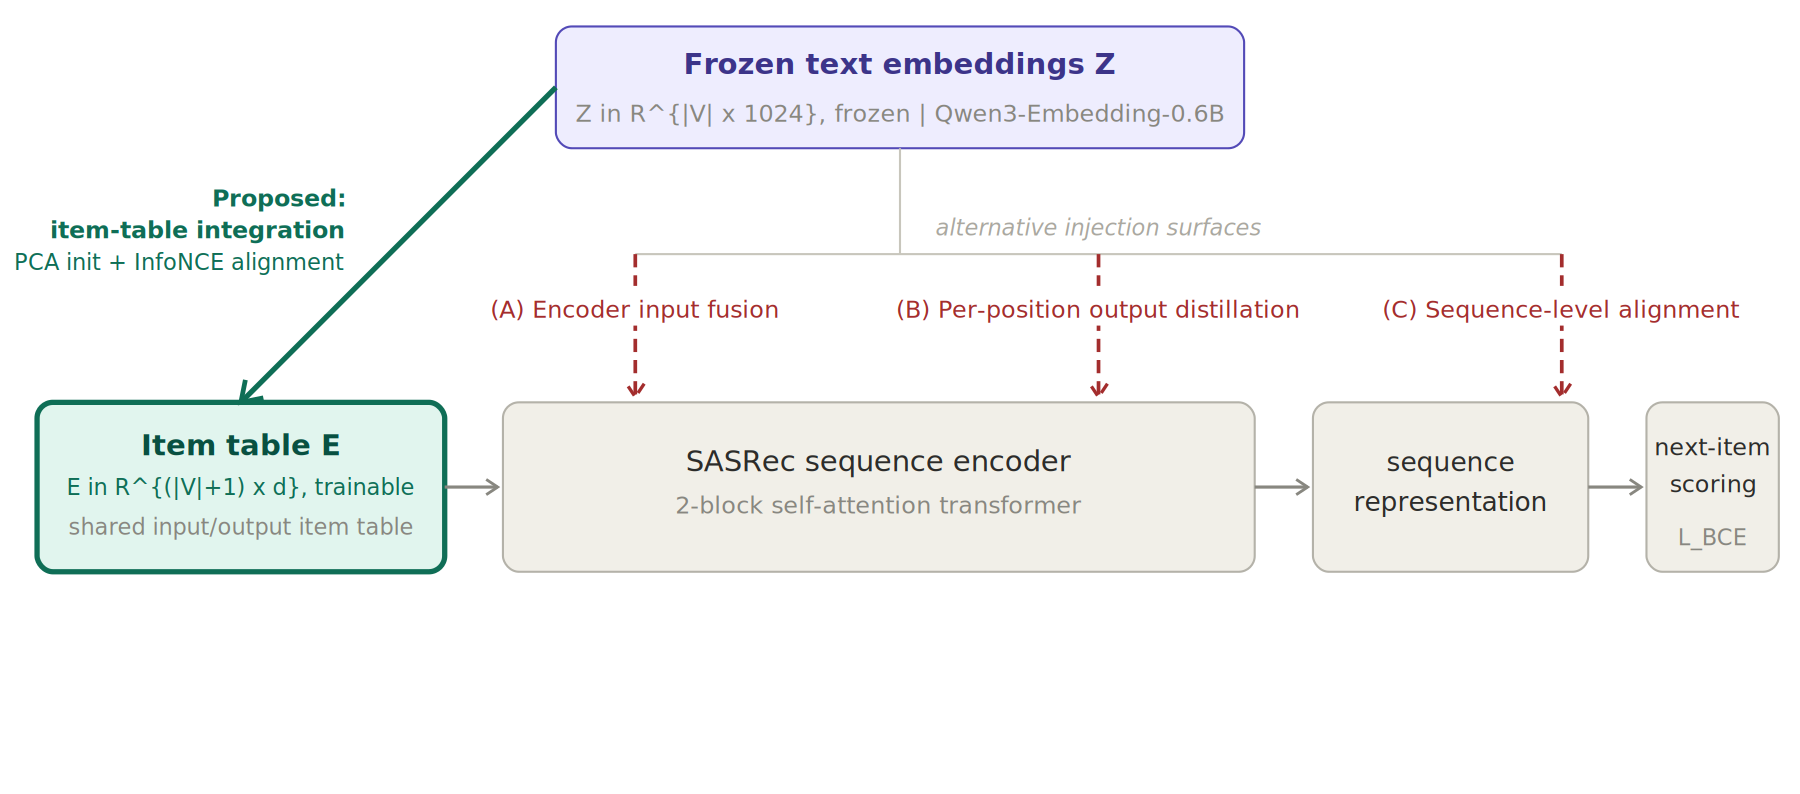
\includegraphics[width=\linewidth]{figures/fig1_surfaces.png}
  }{%
    \fbox{\rule[-.5cm]{0cm}{3cm} \rule[-.5cm]{\linewidth}{0cm}}
  }
  \caption{\textbf{The four semantic injection surfaces studied in this
    work, illustrated on a SASRec backbone.} Frozen text embeddings
    $\mathbf{Z} \in \mathbb{R}^{|\mathcal{V}| \times 1024}$ produced by
    Qwen3-Embedding-0.6B can enter the recommender at four distinct
    points. Dashed red arrows (A--C) inject into the sequence encoder:
    (A)~encoder input fusion, (B)~per-position output distillation, and
    (C)~sequence-level alignment of the final user representation. The
    solid green arrow (ours) shapes the trainable item embedding table
    $\mathbf{E} \in \mathbb{R}^{(|\mathcal{V}|+1) \times d}$ directly,
    leaving the sequence encoder entirely untouched. Because
    $\mathbf{E}$ is shared between input encoding and next-item
    scoring, the proposed item-table integration propagates to
    candidate ranking at inference even though all auxiliary
    parameters are discarded after training.}
  \label{fig:surfaces}
\end{figure}
% ------------------------------------------------------------------

\paragraph{Contributions.}
\begin{enumerate}
  \item A controlled empirical study that isolates the injection
    surface as the experimental variable under a fixed SASRec backbone,
    comparing four representative surfaces and showing that item-table
    integration gives the best aggregate metrics and strongest sampled-tail metrics among the four surfaces studied.
  \item Identification of popularity-dependent effects:
    initialization is the dominant driver of aggregate accuracy
    (concentrated on head items), and item-table InfoNCE alignment
    lifts sampled hit rate for long-tail items that the next-item objective
    neglects. We do not claim recovery on the harder full-rank
    tail regime, where SASRec itself scores at or near zero.
  \item A lightweight item-table framework combining LLM-PCA
    initialization with a symmetric InfoNCE alignment loss, adding no inference-time
    overhead relative to the SASRec backbone.
\end{enumerate}

% -----------------------------------------------------------------------
% TARGET: ~1--1.5 pages
\section{Related Work}

\paragraph{Sequential recommendation.}
Early neural approaches modeled user dynamics with recurrent
networks~\cite{hidasi2016gru4rec}; subsequent work adopted self-attention
as the primary backbone, with SASRec~\cite{kang2018sasrec} using causal
self-attention for next-item prediction and
BERT4Rec~\cite{sun2019bert4rec} adapting bidirectional transformers
through masked item prediction. These models learn collaborative
patterns effectively but rely entirely on behavioral data, leaving item
representations poorly calibrated for sparse items.

\paragraph{Contrastive learning for sequential recommendation.}
Auxiliary self-supervised objectives improve representation robustness
under sparsity via augmented sequence views~\cite{xie2022cl4srec, qiu2022duorec} or frequency-aware
augmentation that avoids disproportionate harm to rare items~\cite{facl}.
Our frequency-weighted alignment shares the latter motivation but
applies pressure at the item embedding table rather than the sequence encoder.

\paragraph{LLM-enhanced sequential recommendation.}
Several systems incorporate LLM-derived signals into sequential
recommenders through different mechanisms.
MoRec~\cite{morec} studies ID- versus modality-based item
representations as competing alternatives;
DLLM2Rec~\cite{dllm2rec} distills LLM ranking signals into a student
recommender, altering the supervision signal rather than the injection
point; LLMEmb~\cite{llmemb} adapts LLM item embeddings through
supervised contrastive fine-tuning and an adapter retained at serving
time; and LLM-ESR~\cite{llmesr}, the closest system to ours in
long-tail motivation, retains frozen semantic embeddings as a deployed
dual-view component alongside the collaborative table. In contrast,
we hold the SASRec backbone fixed and isolate the injection surface as
the experimental variable, then propose an item-table method that
uses frozen text embeddings only to initialize and regularize the
trainable ID table; all auxiliary semantic modules are discarded after training.

% -----------------------------------------------------------------------
% TARGET: ~3 pages
% Cover: problem formulation, SASRec backbone, LLM embedding extraction
%        (Qwen3-Embedding-0.6B), four injection surfaces (A2/A3/A4/A8),
%        LLM-PCA initialization (spectral projection), frequency-weighted
%        InfoNCE loss (math formulation), training algorithm, inference.
\section{Methodology}

% ------------------------------------------------------------------
% FIGURE 2 PLACEHOLDER
% Detailed method diagram for the proposed item-table integration framework.
% Show two components side by side:
%   LEFT — LLM-PCA Initialization:
%     Qwen3 LLM → item text → 1024-dim embeddings → PCA (50-dim)
%     → initialize SASRec item embedding table
%   RIGHT — Frequency-Weighted Contrastive Alignment (training only):
%     SASRec item_emb(ids) + frozen LLM_emb(ids) → linear projector
%     → symmetric InfoNCE loss, weights w_i = 1/(1 + log(freq_i + 1))
%     → combined loss: L_total = L_BCE + λ · L_align
%   BOTTOM — Inference: standard SASRec, no LLM, no projector
% Include the weight function plot (log-inverse curve) as a small inset
% to visually explain why tail items get more pressure.
\begin{figure}[t]
  \centering
  \IfFileExists{figures/fig2_method.png}{%
    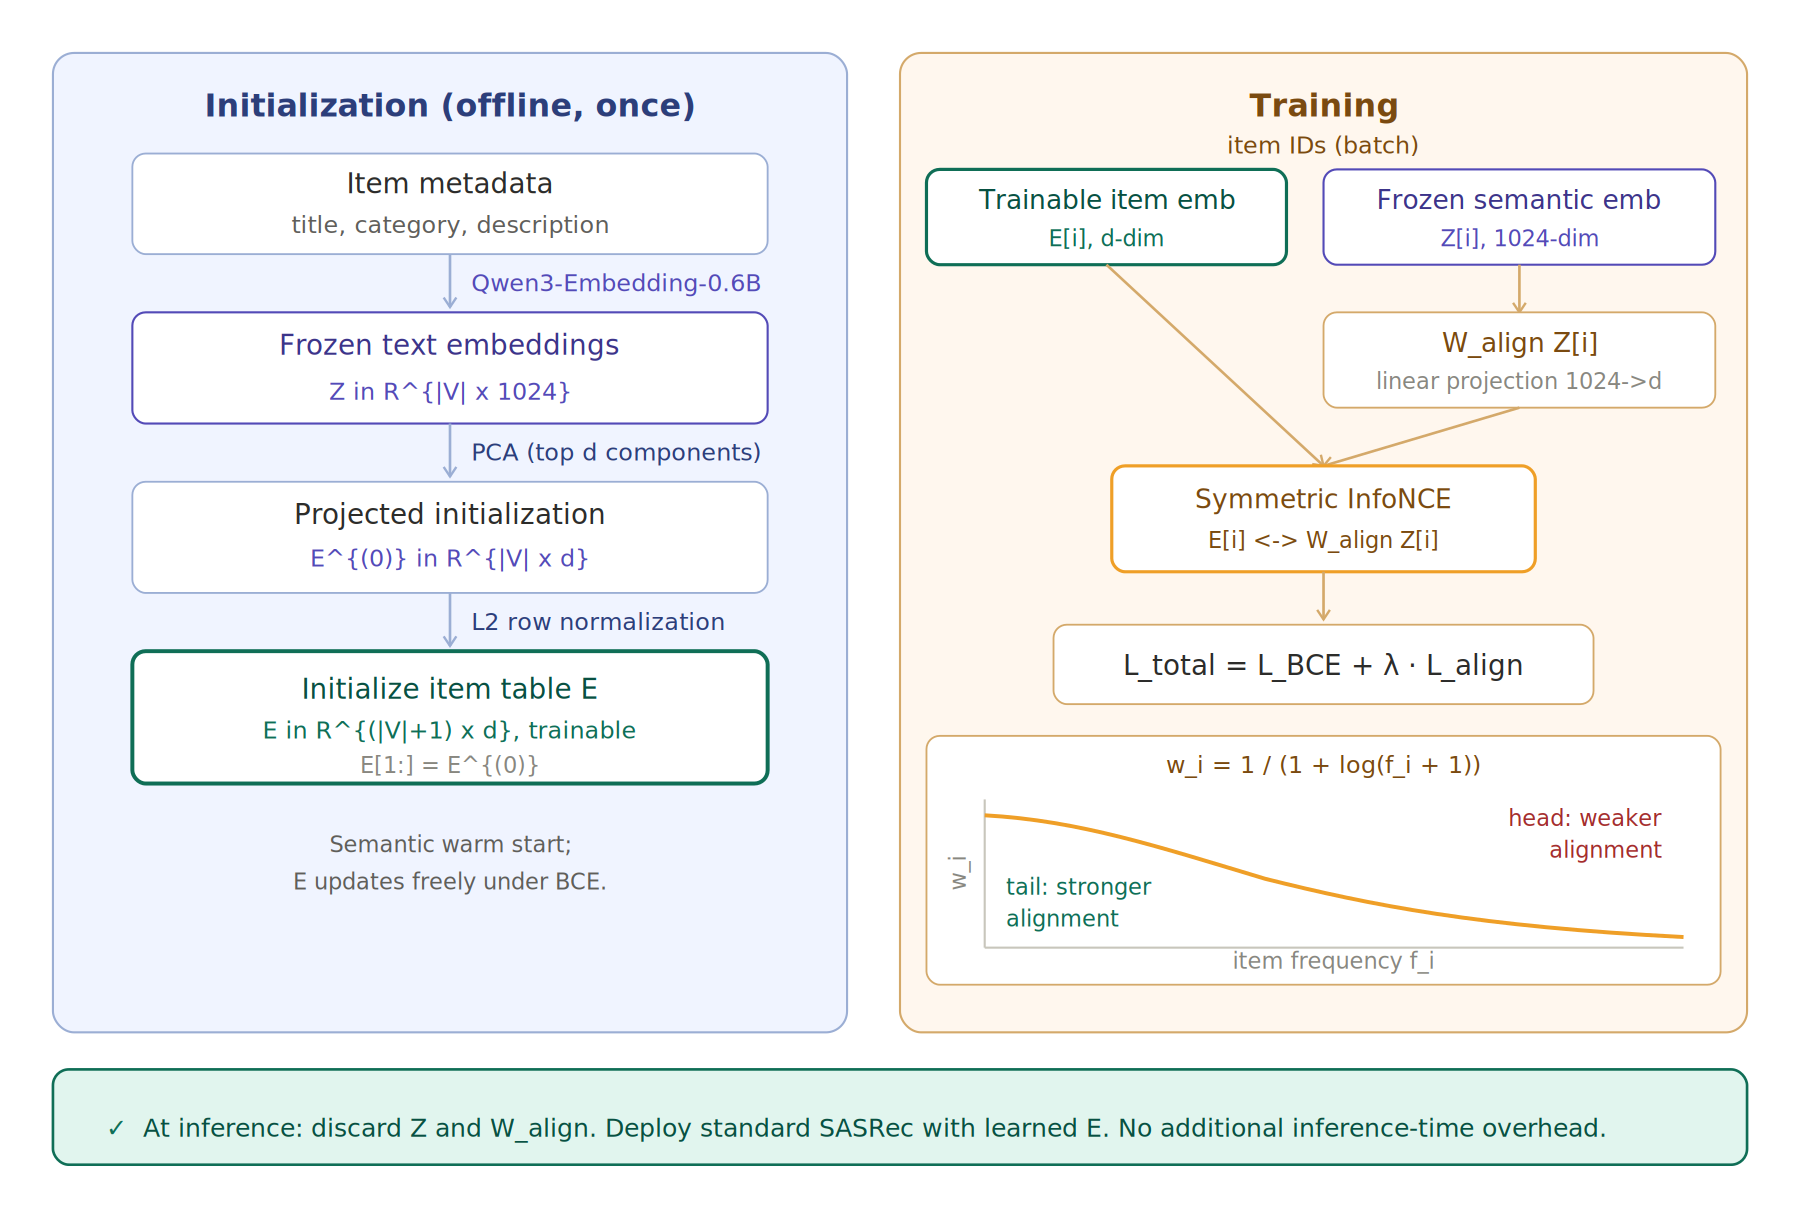
\includegraphics[width=\linewidth]{figures/fig2_method.png}%
  }{%
    \fbox{\rule[-.5cm]{0cm}{5cm} \rule[-.5cm]{12cm}{0cm}}%
  }
  \caption{\textbf{Proposed item-table integration framework.}
    \textit{Left, offline initialization:} item text is encoded
    by frozen Qwen3-Embedding-0.6B to produce $\mathbf{Z}[i] \in \mathbb{R}^{1024}$;
    a centered SVD compresses the catalog to $d = 50$ and seeds the
    trainable item table $\mathbf{E}[i]$ before training.
    \textit{Right, training-time alignment:} for each batch of unique
    item ids, $\mathbf{E}[i]$ and $W_\text{align}\mathbf{Z}[i]$ are
    pulled together by a symmetric InfoNCE loss; per-item weights
    apply stronger pressure to low-frequency items
    (Equation~\ref{eq:freq-weights}).
    \textit{Bottom, inference:} both $\mathbf{Z}$ and $W_\text{align}$
    are discarded and the deployed model is exactly the SASRec
    backbone.}
  \label{fig:method}
\end{figure}
% ------------------------------------------------------------------

\subsection{Problem Formulation and Backbone}

Let $\mathcal{V}$ denote the item catalog with $|\mathcal{V}| = N$
items and, for each user $u$, let
$S_u = (v_1^u, \ldots, v_{T_u}^u)$ be a chronologically ordered
interaction sequence. We use SASRec~\cite{kang2018sasrec} as a unified
backbone across all experiments. An item embedding table
$\mathbf{E} \in \mathbb{R}^{(N+1) \times d}$ (with index $0$ reserved
for padding) and a learned positional embedding produce input
representations $\mathbf{h}^{(0)}_t = \mathbf{E}[v_t] + \mathbf{P}[t]$
that pass through $B$ Transformer blocks with causal self-attention,
yielding per-position output $\mathbf{h}^{(B)}_t \in \mathbb{R}^d$.
We tie the input and output item tables, so $\mathbf{E}$ is used both
for history lookup and candidate scoring via
$s_{t,i} = \mathbf{h}^{(B)\top}_t \mathbf{E}[i]$ (raw dot product).
The padding row $\mathbf{E}[0]$ is fixed at zero and excluded from
PCA fitting, alignment batches, frequency counts, loss computation,
and evaluation. Following the original paper, we use $d = 50$,
$B = 2$ blocks, a single attention head, sequence length $L = 200$,
and dropout $0.2$.

Training uses next-item BCE: for each position $t$ we pair the
ground-truth next item with a uniformly sampled negative (rejected
if it collides with any item in the user's training sequence,
following standard SASRec practice; held-out validation and test
items can in principle appear but the impact is negligible given
catalog sizes of $10^4$--$10^5$) and apply BCE against the
position's score. For each item $v$ we construct a short textual
description from per-dataset metadata fields
(Section~\ref{sec:datasets}; missing fields are omitted, not
placeholdered) and encode it with a frozen Qwen3-Embedding-0.6B
model~\cite{qwen3embed},
producing $\mathbf{Z}[v] \in \mathbb{R}^{1024}$. Embeddings are
L2-normalized at extraction. $\mathbf{Z}$ is precomputed once per
dataset and is not required at serving time.

\subsection{Semantic Injection Surfaces}
\label{sec:surfaces}

We instantiate four injection surfaces in the SASRec backbone
(Figure~\ref{fig:surfaces}). All share the same BCE objective.

\paragraph{(A) Encoder input fusion.}
$\mathbf{h}^{(0)}_t = \mathbf{E}[v_t] + W_\text{in}\, \mathbf{Z}[v_t] + \mathbf{P}[t]$,
where $W_\text{in} \in \mathbb{R}^{d \times d_\text{LLM}}$ is learned;
no auxiliary loss. Unlike the other surfaces, $\mathbf{Z}$ and
$W_\text{in}$ remain on the model at inference (every sequence step
requires a lookup and a $d_\text{LLM} \times d$ matmul).

\paragraph{(B) Per-position output distillation.}
Inspired by knowledge distillation~\cite{hinton2015distill}, a
symmetric InfoNCE loss (temperature $\tau$) aligns
$\mathbf{h}^{(B)}_t$ with $W_\text{out}\, \mathbf{Z}[v_{t+1}^u]$ at
every non-padding position, matching the next-item prediction
target.

\paragraph{(C) Sequence-level alignment.}
A symmetric InfoNCE loss (temperature $\tau$) aligns the final
position output $\mathbf{h}^{(B)}_{L-1}$ (which under left-padding
is the most recent real item's representation) with the mean-pooled
semantic embedding $\frac{1}{T_u}\sum_{t} \mathbf{Z}[v_t^u]$ of the
user's sequence.

\paragraph{Item-table integration (ours).}
The sequence encoder receives no auxiliary signal. $\mathbf{E}$ is
shaped through (i)~a one-time spectral initialization and (ii)~a
training-time symmetric InfoNCE alignment loss, both operating on
the item table only (\S\ref{sec:item-table}). Because
$\mathbf{E}$ is tied between input encoding and output scoring, this
shaping propagates to candidate ranking at inference even though all
auxiliary parameters ($W_\text{align}$, $\mathbf{Z}$) are discarded
after training. Surfaces (B), (C), and the proposed item-table
integration add an auxiliary loss to BCE weighted by $\lambda$;
(A) does not.

\subsection{Item-Table Integration}
\label{sec:item-table}

\paragraph{LLM-PCA initialization.}
\label{sec:llm-pca}
Let $\mathbf{Z} \in \mathbb{R}^{N \times d_\text{LLM}}$ denote the
catalog matrix (padding excluded). After row-wise L2-normalization we
center, decompose
$\tilde{\mathbf{Z}} = U \Sigma V^\top$, and project to the top-$d$
principal axes:
$\mathbf{E}^{(0)} = \mathrm{normalize}\big(\tilde{\mathbf{Z}} V_{:d}\big)$,
re-L2-normalizing each row to unit length. We seed
$\mathbf{E}[1{:}] \gets \mathbf{E}^{(0)}$ and then let $\mathbf{E}$
update freely under BCE. The unit-norm rows differ in magnitude from
the SASRec Xavier-uniform baseline. The PCA fit is offline
and negligible relative to training time.

\paragraph{Frequency-weighted symmetric InfoNCE.}
\label{sec:freq-infonce}
The alignment objective uses the InfoNCE contrastive
loss~\cite{vandenoord2018cpc} applied symmetrically between the
trainable item table and the projected frozen LLM table. Let
$\mathcal{B}$ denote the unique non-padding item ids touched by a
training batch, $|\mathcal{B}| = M$. For each $i \in \mathcal{B}$ we
take $\mathbf{s}_i = \mathbf{E}[i]$ and
$\mathbf{t}_i = W_\text{align}\, \mathbf{Z}[i]$, where
$W_\text{align} \in \mathbb{R}^{d \times d_\text{LLM}}$ is a bias-free
linear projector trained jointly with the model. With L2-normalized
versions $\hat{\mathbf{s}}_i, \hat{\mathbf{t}}_i$ and temperature
$\tau = 0.1$, we form
$\mathbf{L}_{ij} = \hat{\mathbf{s}}_i^\top \hat{\mathbf{t}}_j / \tau$
and apply symmetric cross-entropy:
\begin{equation}
  \mathcal{L}_\text{InfoNCE} = \tfrac{1}{2}\bigl(\mathrm{CE}(\mathbf{L}, \mathbf{I}) + \mathrm{CE}(\mathbf{L}^\top, \mathbf{I})\bigr).
  \label{eq:infonce}
\end{equation}
To weight tail items more strongly we replace the unweighted mean
inside each cross-entropy with a weighted mean using a
non-increasing function of training-set frequency $f_i$,
\begin{equation}
  w_i = g(f_i), \qquad \tilde{w}_i = M \cdot \frac{w_i}{\sum_{j \in \mathcal{B}} w_j},
  \label{eq:freq-weights}
\end{equation}
where $\tilde{w}_i$ normalizes to mean $1$, preserving loss scale
while increasing relative pressure on low-frequency items. We
consider four parameterizations of $g$ (logarithmic, square-root,
linear, and a binary head/tail split) and select between them on
validation full-rank N@10 (Appendix~\ref{app:weight-sweep});
the selected variant is the binary split, $g(f_i) = 2$ for items
in the bottom 20\% of training-set frequency and $g(f_i) = 0.5$
otherwise.

\subsection{Training and Inference}

The total objective combines next-item BCE with the auxiliary alignment
loss,
$\mathcal{L}_\text{total} = \mathcal{L}_\text{BCE} + \lambda \cdot \mathcal{L}_\text{InfoNCE}^{(w)}$,
with $\lambda$ selected on Video Games full-rank N@10
(\S\ref{sec:experimental-setup}). The alignment loss touches only rows
of $\mathbf{E}$ that BCE is already updating, so the additional
per-step cost is dominated by a single $(M, M)$ matrix product. At inference time both $\mathbf{Z}$ and $W_\text{align}$ are
discarded: the deployed model contains only the SASRec parameters,
adding \emph{zero serving overhead}. Offline costs (one LLM forward pass per catalog item, one SVD,
and per-step contrastive products during training) are incurred
once per catalog version and must be re-run when the catalog changes.

% -----------------------------------------------------------------------
% TARGET: ~1--1.5 pages
% Cover: datasets (Video Games, Beauty, Sports, Yelp — statistics table),
%        baseline models (SASRec, CL4SRec, LLM-ESR if available),
%        evaluation metrics (HR@5/10/20, NDCG@5/10/20, full-rank + sampled),
%        popularity stratification protocol (head/torso/tail buckets),
%        hyperparameters, seeds, hardware.
\section{Experimental Setup}
\label{sec:experimental-setup}

\subsection{Datasets}
\label{sec:datasets}

We evaluate on four sequential recommendation benchmarks: three
Amazon Reviews 2023 categories from \citet{hou2024amazon} (Video
Games, Sports and Outdoors, and Beauty and Personal Care), and the
Yelp Open Dataset~\citep{yelpdataset}. For Amazon the LLM-encoder
text input is \texttt{title}~+~\texttt{description}; for Yelp we
reproduce the LLM-ESR~\citep{llmesr} multi-field template
verbatim. Full prompt templates and truncation rules are in
Appendix~\ref{app:prompts}.

\paragraph{Preprocessing.} For Amazon Reviews 2023 we download the
\texttt{benchmark/5core/rating\_only} subsets from
\citet{hou2024amazon}, which are already iterative-bipartite 5-core
fixed points: re-applying the filter drops zero users, items, and
interactions on all three categories. For Yelp we apply iterative
bipartite 5-core to the raw review log, alternating drops of users
and items below five interactions until the table is stable. All
four datasets are chronologically sorted per user and remapped to
contiguous integer ids (id 0 reserved for padding).

\paragraph{Splits.} We use a leave-one-out
split~\citep{kang2018sasrec,sun2019bert4rec}: per-user, the last
interaction is held out for test, the second-to-last for validation,
and the remainder for training. After 5-core no users are dropped
for being too short. Note that 5-core filtering means all evaluated items have at least
five interactions; results speak to \emph{sparse} items within this
set, not true cold-start.

\paragraph{Popularity strata.} For the popularity-stratified
evaluation in Section~\ref{sec:results} we partition items by
\emph{training-set} frequency into head (top 20\%), torso (middle
60\%), and tail (bottom 20\%) buckets. Cuts are computed on the
training split only, so val/test leakage is avoided. All four datasets
are strongly long-tailed: head 20\% of items receive 65--71\% of
training interactions while tail 20\% receive only 2.7--3.9\%.
Table~\ref{tab:datasets} reports per-dataset statistics and
Table~\ref{tab:popularity} the per-bucket breakdown.

\begin{table}[t]
  \centering
  \small
  \caption{Dataset statistics after 5-core preprocessing. The
  \#Interactions column counts the full per-user sequences before
  the leave-one-out split removes two interactions per user.}
  \label{tab:datasets}
  \begin{tabular}{lrrrr}
    \toprule
    Dataset & \#Users & \#Items & \#Interactions & Avg.\ seq.\ len \\
    \midrule
    Video Games               &  94{,}762 &  25{,}612 &    814{,}586 &  8.6 \\
    Sports and Outdoors       & 409{,}772 & 156{,}235 &  3{,}472{,}020 &  8.5 \\
    Beauty and Personal Care  & 729{,}576 & 207{,}649 &  6{,}624{,}441 &  9.1 \\
    Yelp                      & 277{,}631 & 112{,}394 &  4{,}250{,}483 & 15.3 \\
    \bottomrule
  \end{tabular}
\end{table}

\begin{table}[t]
  \centering
  \small
  \caption{Popularity bucket breakdown on the training split. Each
  bucket holds 20\% / 60\% / 20\% of items by training-set frequency
  (i.e.\ after the leave-one-out split removes the val and test
  interactions). \emph{Avg.} is the average number of training
  interactions per item in that bucket; \emph{Share} is the bucket's
  percentage of total training interactions.}
  \label{tab:popularity}
  \begin{tabular}{lrrrrrr}
    \toprule
    & \multicolumn{2}{c}{Head} & \multicolumn{2}{c}{Torso} & \multicolumn{2}{c}{Tail} \\
    \cmidrule(lr){2-3}\cmidrule(lr){4-5}\cmidrule(lr){6-7}
    Dataset & Avg. & Share & Avg. & Share & Avg. & Share \\
    \midrule
    Video Games              &  87.1 & 71.1\% & 10.6 & 26.0\% & 3.5 & 2.8\% \\
    Sports and Outdoors      &  55.2 & 64.9\% &  8.8 & 31.2\% & 3.3 & 3.9\% \\
    Beauty and Personal Care &  87.8 & 70.5\% & 11.0 & 26.4\% & 3.8 & 3.1\% \\
    Yelp                     & 116.6 & 70.9\% & 14.5 & 26.5\% & 4.4 & 2.7\% \\
    \bottomrule
  \end{tabular}
\end{table}

\subsection{Baselines and Evaluation Protocol}
\label{sec:protocol}

\paragraph{Baselines.} Our baseline is
\textbf{SASRec}~\citep{kang2018sasrec} trained with the exact
backbone and recipe used by every variant (Section~\ref{sec:hyperparams}).
All reported numbers come from our pipeline; we do not transcribe
numbers from prior work because our preprocessing, sampled-eval
seed pool, and full-rank protocol are end-to-end controlled, and
direct comparison would conflate method differences with protocol
differences. Surfaces (A)--(C) in Table~\ref{tab:surfaces}
represent the main architectural locations at which prior
LLM-enhanced systems introduce semantic representations,
re-implemented here under our shared backbone.

\paragraph{Metrics.} We report H@$k$ and N@$k$ for $k \in \{5,
10, 20\}$ under two ranking protocols. \textbf{Sampled@100} follows
the standard SASRec-style sampled-negative
evaluation~\citep{kang2018sasrec}: each held-out target is ranked
against 100 uniform-random negatives drawn once per user with a
fixed seed and cached to disk, with the user's full sequence
(train+val+test items) rejected from the negative pool. Sampled
metrics are paired, so every variant ranks the same target against
the same 100 negatives and variance reflects model differences
rather than negative-pool differences. \textbf{Full-rank}: each
target is ranked against all $N$ catalog items with the user's
training items and held-out validation item masked from the
candidate set (the test target itself remains rankable). Scores
are computed in mini-batches of users to bound memory on catalogs
with $N > 10^5$. Full-rank metrics are much
smaller in absolute magnitude than sampled metrics on large
catalogs. We report both.

\paragraph{Validation and early stopping.} Validation N@10
(sampled) is computed every epoch; training stops when validation
has not improved by more than $10^{-3}$ for 10 consecutive epochs.
The same criterion is applied across all datasets and all variants.

\subsection{Hyperparameters and Hyperparameter Search}
\label{sec:hyperparams}

\paragraph{SASRec backbone (shared by all variants).} We use the
canonical SASRec~\citep{kang2018sasrec} configuration: $d=50$,
two transformer blocks, single attention head, $L=200$, dropout 0.2;
item embeddings are tied between input and output.
Optimization: Adam~\cite{kingma2014adam}, lr $10^{-3}$,
batch 512, up to 200 epochs with early stopping (Section~\ref{sec:protocol}).

\paragraph{LLM encoder.} Qwen3-Embedding-0.6B~\citep{qwen3embed},
frozen, producing 1024-dimensional vectors. Encoder weights are
never updated; the LLM is not invoked at inference.

\paragraph{Item-table integration (proposed).} The PCA initialization
keeps the top $d=50$ singular components of the L2-normalized
catalog matrix and re-normalizes each row to unit length. PCA is
chosen over a learned projection because it is parameter-free and
directly targets the principal directions of the frozen LLM space.
The alignment projector is a single bias-free linear map
$\mathbf{W}_{\!\text{align}} \in \mathbb{R}^{d \times d_\text{LLM}}$
with input dropout 0.1. Symmetric InfoNCE makes the alignment
bidirectional, pulling the collaborative table toward the LLM
geometry and the projection toward the collaborative geometry,
without requiring a teacher-student asymmetry. The contrastive
temperature is fixed at $\tau = 0.1$ throughout. The alignment weight $\lambda$
and the frequency-weighting function $g$ are selected on
Video Games full-rank N@10 over the grid
$\lambda \in \{0.01, 0.05, 0.1, 0.5, 1.0\} \times g \in \{\text{log,
sqrt, linear, binary}\}$; the selected configuration ($\lambda =
0.5$, $g = \text{binary}$) is used across all four datasets. The
binary split ($2\times$ for tail, $0.5\times$ otherwise) is
interpretable and minimal; Appendix~\ref{app:weight-sweep} confirms
it is competitive with smoother alternatives. We use full-rank
rather than sampled@100 as the model-selection criterion to avoid
overfitting to the fixed 100-negative pool. To keep alignment
mini-batches tractable, batches with more than $4{,}096$ unique
item ids subsample to $4{,}096$; remaining ids backpropagate only
through BCE. Per-batch weight normalization follows
Equation~\ref{eq:freq-weights}.

\paragraph{Other surfaces.} Surfaces (A), (B), and (C) use the
same backbone and reuse the same $\tau = 0.1$ where applicable.
Each surface's auxiliary loss weight is searched independently on
Video Games N@10 from the same grid.

\subsection{Reproducibility}
\label{sec:reproducibility}

All variants are trained with three random seeds $\{7, 18, 42\}$;
we report mean $\pm$ std. The sampled-eval negative pool and LLM
item embeddings are generated once per dataset and reused across
all variants and seeds. Code, configs, and preprocessing scripts
are available upon request.

\section{Results and Analysis}
\label{sec:results}

% Numbers reported here are 3-seed (seeds 7, 18, 42) means $\pm$ std.

\paragraph{Where should LLM knowledge enter?}
Table~\ref{tab:surfaces} compares the four injection surfaces under
the shared SASRec backbone on Video Games. Item-table integration
(ours) gives the best aggregate metrics on both sampled and
full-rank protocols and the best tail-item metrics, while adding
\emph{zero} parameters at inference. Per-position distillation (B)
is a close competitor: it ties on the second-best aggregate full-rank
H@10 and slightly outperforms our method on full-rank head-item
H@10 / N@10, but trails substantially on tail items. Input fusion
(A) lifts vanilla SASRec slightly but keeps the LLM lookup and
projector at serving cost. Sequence-level alignment (C) is the
weakest: aligning one user-summary vector against a mean-pooled
semantic embedding does not propagate strongly to per-item scores.
The injection surface materially affects performance even under a
fixed backbone, LLM encoder, and tuning grid; among the four, only
item-table integration combines competitive aggregate accuracy
with a clear tail advantage.

\begin{table}[!htbp]
  \centering
  \footnotesize
  \caption{Cross-surface comparison on Video Games. \textsc{Smp}:
  sampled@100; \textsc{Full}: full-rank ($N{=}25{,}612$).
  \textbf{Bold}: best per (column, protocol);
  \underline{underline}: second best. Mean $\pm$ std over seeds
  $\{7,18,42\}$.}
  \label{tab:surfaces}
  \setlength{\tabcolsep}{3pt}
  \resizebox{\linewidth}{!}{%
  \begin{tabular}{llrrrrrr}
    \toprule
    & & \multicolumn{2}{c}{Overall} & \multicolumn{2}{c}{Head item} & \multicolumn{2}{c}{Tail item} \\
    \cmidrule(lr){3-4}\cmidrule(lr){5-6}\cmidrule(lr){7-8}
    Method & Eval & H@10 & N@10 & H@10 & N@10 & H@10 & N@10 \\
    \midrule
    \multirow{2}{*}{SASRec}                           & \textsc{Smp}  & 0.7194{\tiny$\pm$.0021} & 0.4954{\tiny$\pm$.0014} & 0.8719{\tiny$\pm$.0004} & 0.6349{\tiny$\pm$.0009} & 0.2263{\tiny$\pm$.0052} & 0.1087{\tiny$\pm$.0016} \\
                                                       & \textsc{Full} & 0.0574{\tiny$\pm$.0013} & 0.0300{\tiny$\pm$.0006} & 0.0862{\tiny$\pm$.0019} & 0.0452{\tiny$\pm$.0012} & \underline{0.0004}{\tiny$\pm$.0003} & \underline{0.0002}{\tiny$\pm$.0002} \\
    \cmidrule(lr){1-8}
    \multirow{2}{*}{Input fusion (A)}                 & \textsc{Smp}  & 0.7324{\tiny$\pm$.0016} & 0.5069{\tiny$\pm$.0020} & 0.8750{\tiny$\pm$.0016} & 0.6420{\tiny$\pm$.0031} & 0.2539{\tiny$\pm$.0070} & \underline{0.1190}{\tiny$\pm$.0039} \\
                                                       & \textsc{Full} & 0.0595{\tiny$\pm$.0018} & 0.0306{\tiny$\pm$.0010} & 0.0892{\tiny$\pm$.0031} & 0.0461{\tiny$\pm$.0018} & 0.0004{\tiny$\pm$.0001} & 0.0002{\tiny$\pm$.0001} \\
    \cmidrule(lr){1-8}
    \multirow{2}{*}{Per-position InfoNCE (B)}         & \textsc{Smp}  & \underline{0.7431}{\tiny$\pm$.0023} & \underline{0.5255}{\tiny$\pm$.0016} & \underline{0.8796}{\tiny$\pm$.0039} & \textbf{0.6695}{\tiny$\pm$.0043} & \underline{0.2643}{\tiny$\pm$.0133} & 0.1174{\tiny$\pm$.0089} \\
                                                       & \textsc{Full} & \underline{0.0764}{\tiny$\pm$.0016} & \underline{0.0405}{\tiny$\pm$.0009} & \textbf{0.1171}{\tiny$\pm$.0022} & \textbf{0.0623}{\tiny$\pm$.0013} & 0.0001{\tiny$\pm$.0001} & 0.0000{\tiny$\pm$.0000} \\
    \cmidrule(lr){1-8}
    \multirow{2}{*}{Sequence-level InfoNCE (C)}       & \textsc{Smp}  & 0.7183{\tiny$\pm$.0013} & 0.4938{\tiny$\pm$.0004} & 0.8717{\tiny$\pm$.0010} & 0.6346{\tiny$\pm$.0009} & 0.2232{\tiny$\pm$.0019} & 0.1063{\tiny$\pm$.0028} \\
                                                       & \textsc{Full} & 0.0575{\tiny$\pm$.0002} & 0.0304{\tiny$\pm$.0000} & 0.0869{\tiny$\pm$.0004} & 0.0462{\tiny$\pm$.0001} & 0.0003{\tiny$\pm$.0001} & 0.0001{\tiny$\pm$.0001} \\
    \cmidrule(lr){1-8}
    \multirow{2}{*}{\textbf{Item-table (ours)}}       & \textsc{Smp}  & \textbf{0.7539}{\tiny$\pm$.0009} & \textbf{0.5339}{\tiny$\pm$.0005} & \textbf{0.8834}{\tiny$\pm$.0015} & \underline{0.6692}{\tiny$\pm$.0021} & \textbf{0.3195}{\tiny$\pm$.0079} & \textbf{0.1512}{\tiny$\pm$.0030} \\
                                                       & \textsc{Full} & \textbf{0.0775}{\tiny$\pm$.0005} & \textbf{0.0412}{\tiny$\pm$.0004} & \underline{0.1160}{\tiny$\pm$.0009} & \underline{0.0620}{\tiny$\pm$.0006} & \textbf{0.0022}{\tiny$\pm$.0003} & \textbf{0.0010}{\tiny$\pm$.0001} \\
    \bottomrule
  \end{tabular}}%
\end{table}

\paragraph{Cross-dataset generalization.}
Table~\ref{tab:main} tests whether the winning surface generalises
beyond the development benchmark. Item-table integration improves over SASRec on every
sampled-protocol cell across all three datasets, and on Sports
and Beauty it wins every full-rank cell as well, a clean
sweep across two short-sequence Amazon catalogs. Yelp shows the
same sampled-protocol pattern (including a $1.3\times$ sampled tail
lift), though full-rank metrics are noisier given that SASRec
already scores near zero on Yelp tail items.

\begin{table}[!htbp]
  \centering
  \footnotesize
  \caption{Cross-dataset generalization beyond Video Games:
  SASRec vs.\ item-table integration on three additional benchmarks.
  Reported under both \textsc{Smp}\,=\,sampled@100 and
  \textsc{Full}\,=\,full-rank ranking. \textbf{Bold} marks the
  within-dataset best per (column, protocol). Mean $\pm$ std over
  seeds $\{7, 18, 42\}$.}
  \label{tab:main}
  \setlength{\tabcolsep}{3pt}
  \resizebox{\linewidth}{!}{%
  \begin{tabular}{llcrrrrrr}
    \toprule
    & & & \multicolumn{2}{c}{Overall} & \multicolumn{2}{c}{Head item} & \multicolumn{2}{c}{Tail item} \\
    \cmidrule(lr){4-5}\cmidrule(lr){6-7}\cmidrule(lr){8-9}
    Dataset & Method & Eval & H@10 & N@10 & H@10 & N@10 & H@10 & N@10 \\
    \midrule
    \multirow{4}{*}{Sports}  & \multirow{2}{*}{SASRec}             & \textsc{Smp}  & 0.6290{\tiny$\pm$.0021} & 0.4041{\tiny$\pm$.0020} & 0.8146{\tiny$\pm$.0021} & 0.5569{\tiny$\pm$.0024} & 0.1775{\tiny$\pm$.0070} & 0.0795{\tiny$\pm$.0063} \\
                              &                                     & \textsc{Full} & 0.0101{\tiny$\pm$.0006} & 0.0051{\tiny$\pm$.0004} & 0.0168{\tiny$\pm$.0011} & 0.0085{\tiny$\pm$.0007} & 0.0000{\tiny$\pm$.0000} & 0.0000{\tiny$\pm$.0000} \\
                              & \multirow{2}{*}{Item-table (ours)}  & \textsc{Smp}  & \textbf{0.6862}{\tiny$\pm$.0008} & \textbf{0.4634}{\tiny$\pm$.0003} & \textbf{0.8474}{\tiny$\pm$.0016} & \textbf{0.6170}{\tiny$\pm$.0024} & \textbf{0.2947}{\tiny$\pm$.0066} & \textbf{0.1368}{\tiny$\pm$.0039} \\
                              &                                     & \textsc{Full} & \textbf{0.0193}{\tiny$\pm$.0005} & \textbf{0.0100}{\tiny$\pm$.0003} & \textbf{0.0319}{\tiny$\pm$.0009} & \textbf{0.0166}{\tiny$\pm$.0005} & \textbf{0.0003}{\tiny$\pm$.0000} & \textbf{0.0001}{\tiny$\pm$.0000} \\
    \midrule
    \multirow{4}{*}{Beauty}  & \multirow{2}{*}{SASRec}             & \textsc{Smp}  & 0.6780{\tiny$\pm$.0075} & 0.4560{\tiny$\pm$.0065} & 0.8412{\tiny$\pm$.0069} & 0.5893{\tiny$\pm$.0077} & 0.1014{\tiny$\pm$.0050} & 0.0437{\tiny$\pm$.0018} \\
                              &                                     & \textsc{Full} & 0.0136{\tiny$\pm$.0009} & 0.0070{\tiny$\pm$.0006} & 0.0192{\tiny$\pm$.0013} & 0.0099{\tiny$\pm$.0009} & 0.0000{\tiny$\pm$.0000} & 0.0000{\tiny$\pm$.0000} \\
                              & \multirow{2}{*}{Item-table (ours)}  & \textsc{Smp}  & \textbf{0.7345}{\tiny$\pm$.0016} & \textbf{0.5151}{\tiny$\pm$.0012} & \textbf{0.8799}{\tiny$\pm$.0008} & \textbf{0.6474}{\tiny$\pm$.0008} & \textbf{0.1952}{\tiny$\pm$.0025} & \textbf{0.0909}{\tiny$\pm$.0014} \\
                              &                                     & \textsc{Full} & \textbf{0.0216}{\tiny$\pm$.0002} & \textbf{0.0114}{\tiny$\pm$.0002} & \textbf{0.0304}{\tiny$\pm$.0002} & \textbf{0.0160}{\tiny$\pm$.0002} & \textbf{0.0002}{\tiny$\pm$.0001} & \textbf{0.0001}{\tiny$\pm$.0000} \\
    \midrule
    \multirow{4}{*}{Yelp}    & \multirow{2}{*}{SASRec}             & \textsc{Smp}  & 0.9096{\tiny$\pm$.0007} & 0.7026{\tiny$\pm$.0007} & 0.9656{\tiny$\pm$.0003} & 0.8027{\tiny$\pm$.0006} & 0.6132{\tiny$\pm$.0013} & 0.3328{\tiny$\pm$.0013} \\
                              &                                     & \textsc{Full} & \textbf{0.0432}{\tiny$\pm$.0005} & \textbf{0.0239}{\tiny$\pm$.0004} & 0.0577{\tiny$\pm$.0008} & 0.0307{\tiny$\pm$.0007} & \textbf{0.0113}{\tiny$\pm$.0009} & \textbf{0.0081}{\tiny$\pm$.0006} \\
                              & \multirow{2}{*}{Item-table (ours)}  & \textsc{Smp}  & \textbf{0.9344}{\tiny$\pm$.0011} & \textbf{0.7147}{\tiny$\pm$.0032} & \textbf{0.9674}{\tiny$\pm$.0005} & \textbf{0.8104}{\tiny$\pm$.0012} & \textbf{0.7828}{\tiny$\pm$.0064} & \textbf{0.4075}{\tiny$\pm$.0084} \\
                              &                                     & \textsc{Full} & 0.0432{\tiny$\pm$.0010} & 0.0223{\tiny$\pm$.0006} & \textbf{0.0642}{\tiny$\pm$.0011} & \textbf{0.0329}{\tiny$\pm$.0006} & 0.0027{\tiny$\pm$.0007} & 0.0016{\tiny$\pm$.0005} \\
    \bottomrule
  \end{tabular}}%
\end{table}

\paragraph{Inside item-table integration.}
Table~\ref{tab:decomp} walks the $\langle$init, alignment,
weighting$\rangle$ space on Video Games. The overall H@10 columns
show that \emph{initialization is the dominant lever}: LLM-PCA
init lifts sampled overall H@10 from $0.7194$ to $0.7522$, and no
subsequent combination of alignment or weighting moves overall
H@10 by more than $\pm 0.003$. The tail columns tell the
complementary story: init alone lifts sampled tail from $0.2263$
to $0.2848$, but combining it with frequency-weighted InfoNCE
alignment goes furthest, reaching sampled tail H@10 of $0.3195$.
The two ingredients act on orthogonal axes: init dominates overall
accuracy, frequency-weighted alignment dominates the sampled-tail
lift. Figure~\ref{fig:stratified} visualizes the head/torso/tail
breakdown.

\begin{table}[!htbp]
  \centering
  \footnotesize
  \caption{Item-table integration decomposition on Video Games.
  ``Init'' is Xavier (vanilla) vs LLM-PCA; ``Align'' is whether
  the symmetric InfoNCE alignment loss is attached to the item
  table; ``Weight'' is the alignment weighting scheme. Overall
  H@10 is mostly determined by initialization; the tail metric is
  where alignment, and specifically frequency weighting on top of
  LLM-PCA, makes the difference. Mean $\pm$ std over seeds
  $\{7, 18, 42\}$.}
  \label{tab:decomp}
  \setlength{\tabcolsep}{4pt}
  \resizebox{\linewidth}{!}{%
  \begin{tabular}{lllrrrr}
    \toprule
    & & & \multicolumn{2}{c}{Sampled@100} & \multicolumn{2}{c}{Full-rank} \\
    \cmidrule(lr){4-5}\cmidrule(lr){6-7}
    Init & Align & Weight & Overall H@10 & Tail H@10 & Overall H@10 & Tail H@10 \\
    \midrule
    Xavier  & ---     & ---     & 0.7194{\tiny$\pm$.0021} & 0.2263{\tiny$\pm$.0052} & 0.0574{\tiny$\pm$.0013} & 0.0004{\tiny$\pm$.0003} \\
    LLM-PCA & ---     & ---     & 0.7522{\tiny$\pm$.0009} & 0.2848{\tiny$\pm$.0060} & \textbf{0.0776}{\tiny$\pm$.0008} & 0.0003{\tiny$\pm$.0002} \\
    Xavier  & InfoNCE & uniform & \textbf{0.7572}{\tiny$\pm$.0016} & 0.3114{\tiny$\pm$.0031} & 0.0722{\tiny$\pm$.0002} & 0.0021{\tiny$\pm$.0004} \\
    LLM-PCA & InfoNCE & uniform & \underline{0.7556}{\tiny$\pm$.0009} & 0.3116{\tiny$\pm$.0019} & 0.0713{\tiny$\pm$.0009} & 0.0013{\tiny$\pm$.0003} \\
    Xavier  & InfoNCE & freq    & 0.7446{\tiny$\pm$.0012} & \underline{0.3153}{\tiny$\pm$.0017} & 0.0718{\tiny$\pm$.0011} & \textbf{0.0037}{\tiny$\pm$.0003} \\
    \textbf{LLM-PCA} & \textbf{InfoNCE} & \textbf{freq (ours)} & 0.7539{\tiny$\pm$.0009} & \textbf{0.3195}{\tiny$\pm$.0079} & \underline{0.0775}{\tiny$\pm$.0005} & \underline{0.0022}{\tiny$\pm$.0003} \\
    \bottomrule
  \end{tabular}}%
\end{table}

\paragraph{Popularity stratification.}
Under sampled@100, where absolute numbers are interpretable,
item-table integration lifts Video Games tail H@10 from
$0.2263$ (SASRec) to $0.3195$, a $1.4\times$ relative improvement
on top of an already non-trivial baseline; head items move
slightly from $0.8719$ to $0.8834$.
Figure~\ref{fig:stratified} visualizes the sampled@100
head/torso/tail breakdown across decomposition configurations.
LLM-PCA init lifts head and torso items; frequency-weighted
alignment without LLM-PCA init pushes the tail further but
at a slight head cost. Item-table integration achieves the
best sampled tail (0.3195) while maintaining stronger head
performance than any other configuration that reaches
comparable tail lift.

\begin{figure}[!htbp]
  \centering
  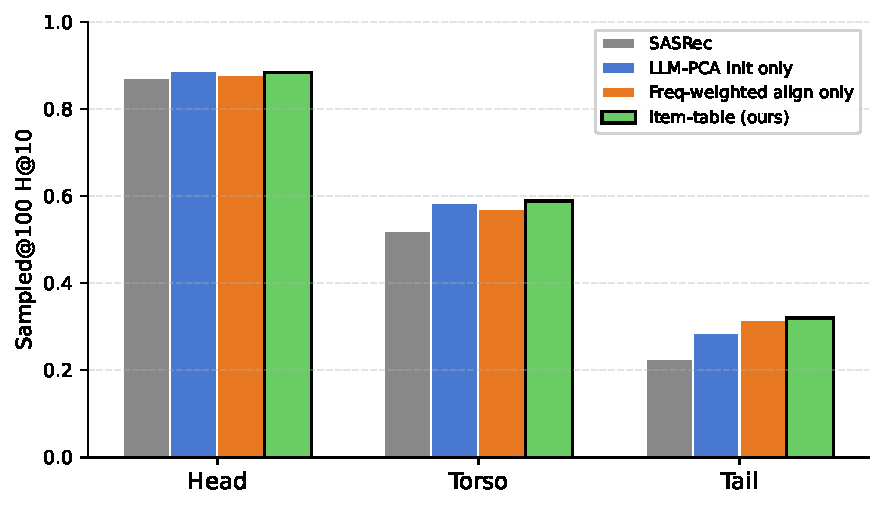
\includegraphics[width=0.78\linewidth]{figures/fig3_stratified.pdf}
  \caption{Sampled@100 H@10 on Video Games stratified by item
  popularity (head 20\% / torso 60\% / tail 20\% by training
  frequency). LLM-PCA initialization lifts head and torso items;
  frequency-weighted alignment alone lifts the tail further but
  slightly reduces head; item-table integration achieves the
  highest tail while maintaining strong head performance.}
  \label{fig:stratified}
\end{figure}

\paragraph{Robustness.}
We additionally swept $\lambda \in \{0.01, 0.05, 0.1, 0.5, 1.0\}$
and the weighting function $g \in \{\text{log, sqrt, linear,
binary}\}$. All four weight functions beat
vanilla SASRec on Video Games full-rank H@10; the three
sub-logarithmic variants (binary, linear, sqrt) further beat the
strongest non-item-table surface (B). Detailed sweep tables are
in Appendix~\ref{app:weight-sweep} and~\ref{app:lambda-sweep}.
Marginal full-rank differences between surfaces (e.g.\ $0.0775$
vs.\ $0.0764$) are close to seed variance and should be interpreted
cautiously.

\FloatBarrier

% -----------------------------------------------------------------------
% TARGET: ~0.5--0.7 page
% Cover: summary of findings, design implications, limitations, future
%        work (BERT4Rec generalization, hybrid POC-2+A8, larger LLM).
\section{Conclusion and Limitations}

We isolated the \emph{semantic injection surface} as the experimental
variable for incorporating frozen LLM embeddings into a sequential
recommender. Under a shared SASRec backbone, item-table integration
gives the best aggregate and sampled-tail metrics among the four
surfaces studied, with zero inference overhead. Item-table
integration is uniquely effective because $\mathbf{E}$ is shared
between input encoding and candidate scoring, so shaping it
propagates semantic structure to ranking without any retained
auxiliary parameters.

The mechanism decomposition shows that LLM-PCA initialization is
the dominant lever for aggregate accuracy while also providing a
meaningful sampled-tail lift; frequency-weighted InfoNCE alignment
pushes the tail further to the best result of any configuration,
with the combination preserving strong aggregate performance.
These findings transfer across Sports, Beauty, and Yelp; we do not
claim recovery in the full-rank tail regime, where SASRec itself
scores near zero on three of four datasets.

\paragraph{Limitations.}
(i)~Results are specific to SASRec ($d{=}50$); other backbones or
larger $d$ may reorder the surfaces.
(ii)~All results use Qwen3-Embedding-0.6B; the ranking may shift
with encoders of different capacity, as each surface's benefit
depends on encoder--collaborative geometry alignment.
(iii)~The method requires item text and must re-run embeddings and
SVD when the catalog changes.

{\small
\begin{thebibliography}{99}

\bibitem[Hidasi et~al.(2016)]{hidasi2016gru4rec}
B.~Hidasi, A.~Karatzoglou, L.~Baltrunas, and D.~Tikk.
Session-based recommendations with recurrent neural networks.
\emph{ICLR}, 2016.

\bibitem[Kang and McAuley(2018)]{kang2018sasrec}
W.-C.~Kang and J.~McAuley.
Self-attentive sequential recommendation.
\emph{ICDM}, 2018.

\bibitem[Sun et~al.(2019)]{sun2019bert4rec}
F.~Sun et al.
BERT4Rec: Sequential recommendation with bidirectional encoder
representations from transformer.
\emph{CIKM}, 2019.

\bibitem[Xie et~al.(2022)]{xie2022cl4srec}
X.~Xie et al.
Contrastive learning for sequential recommendation.
\emph{ICDE}, 2022.

\bibitem[Liu et~al.(2021)]{liu2021coseRec}
Z.~Liu et al.
Contrastive self-supervised sequential recommendation with robust augmentation.
\emph{arXiv}, 2021.

\bibitem[Qiu et~al.(2022)]{qiu2022duorec}
R.~Qiu et al.
Contrastive learning for representation degeneration problem in sequential recommendation.
\emph{WSDM}, 2022.

\bibitem[Wang et~al.(2025)]{wang2024rcl}
Z.~Wang et al.
Relative contrastive learning for sequential recommendation with
similarity-based positive pair selection.
arXiv:2504.19178, 2025.

\bibitem[Wang and Zhang(2026)]{facl}
Z.~Wang and W.~Zhang.
Frequency-aware adaptive contrastive learning for sequential
recommendation.
arXiv:2601.17057, 2026.

\bibitem[Yuan et~al.(2023)]{morec}
Y.~Yuan, G.~Zhang, X.~Liu, J.~Wu, Y.~Wang, M.~Li, and J.~Shi.
Where to go next for recommender systems? ID- vs. modality-based
recommender models revisited.
\emph{SIGIR}, 2023.

\bibitem[Cui et~al.(2024)]{dllm2rec}
Y.~Cui, F.~Liu, P.~Wang, B.~Wang, H.~Tang, Y.~Wan, J.~Wang, and
J.~Chen.
Distillation matters: Empowering sequential recommenders to match
the performance of large language models.
arXiv:2405.00338, 2024.

\bibitem[Liu et~al.(2025)]{llmemb}
Q.~Liu, X.~Wu, Y.~Wang, Z.~Zhang, F.~Tian, Y.~Zheng, and X.~Zhao.
LLMEmb: Large language model can be a good embedding generator for
sequential recommendation.
\emph{AAAI}, 2025. arXiv:2409.19925.

\bibitem[Liu et~al.(2024)]{llmesr}
Q.~Liu, X.~Wu, Y.~Wang, Z.~Zhang, F.~Tian, Y.~Zheng, and X.~Zhao.
LLM-ESR: Large language models enhancement for long-tailed sequential
recommendation.
\emph{NeurIPS}, 2024. arXiv:2405.20646.

\bibitem[Zhang et~al.(2025)]{qwen3embed}
Y.~Zhang, M.~Li, D.~Long, X.~Zhang, H.~Lin, B.~Yang, P.~Xie, A.~Yang,
D.~Liu, J.~Lin, F.~Huang, and J.~Zhou.
Qwen3 embedding: Advancing text embedding and reranking through
foundation models.
arXiv:2506.05176, 2025.

\bibitem[Hou et~al.(2024)]{hou2024amazon}
Y.~Hou, J.~Li, Z.~He, A.~Yan, X.~Chen, and J.~McAuley.
Bridging language and items for retrieval and recommendation.
arXiv:2403.03952, 2024.

\bibitem[Yelp~Inc.(2024)]{yelpdataset}
Yelp~Inc.
Yelp Open Dataset.
\url{https://www.yelp.com/dataset}, 2024.

\bibitem[van~den Oord et~al.(2018)]{vandenoord2018cpc}
A.~van~den Oord, Y.~Li, and O.~Vinyals.
Representation learning with contrastive predictive coding.
arXiv:1807.03748, 2018.

\bibitem[Rajput et~al.(2023)]{rajput2023tiger}
S.~Rajput, N.~Mehta, A.~Singh, R.~Hulikal Keshavan, T.~Vu, L.~Heldt,
L.~Hong, Y.~Tay, V.~Q.~Tran, J.~Samost, M.~Kula, E.~H.~Chi, and
M.~Sathiamoorthy.
Recommender systems with generative retrieval.
\emph{NeurIPS}, 2023.

\bibitem[Kingma and Ba(2015)]{kingma2014adam}
D.~P.~Kingma and J.~Ba.
Adam: A method for stochastic optimization.
\emph{ICLR}, 2015. arXiv:1412.6980.

\bibitem[Hinton et~al.(2015)]{hinton2015distill}
G.~Hinton, O.~Vinyals, and J.~Dean.
Distilling the knowledge in a neural network.
\emph{NeurIPS Deep Learning Workshop}, 2015. arXiv:1503.02531.

\end{thebibliography}
}

\clearpage
\appendix
\section{Prompt templates}
\label{app:prompts}

Each item is encoded once with frozen Qwen3-Embedding-0.6B and the
resulting 1024-dimensional vector is cached. Prompt templates are
short, contain only fields available in the published dataset
metadata, and were not tuned on validation; we expect prompt
sensitivity to be a useful direction for future work.

\paragraph{Amazon Reviews 2023.} Each item is formatted as
$\texttt{<title>}\;\text{---}\;\texttt{<description>}$. The
description is truncated at the last whitespace before 600
characters ($\approx$~150 tokens) so a 10-item sequence stays
under Qwen3's 32K-token context. Items with empty
description fall back to \texttt{<title>}; items with empty title
fall back to the literal string \texttt{Untitled}. Example:

\begin{quote}\small\ttfamily
Street Fighter 30th Anniversary Collection - Nintendo Switch
Standard Edition --- Celebrate the 30th Anniversary of the iconic
Street Fighter franchise with the ultimate tribute to its arcade
legacy in the Street Fighter 30th Anniversary Collection.
\end{quote}

\paragraph{Yelp.} We reproduce the LLM-ESR~\citep{llmesr} template
verbatim. Each business is formatted as:

\begin{quote}\small\ttfamily
The point of interest has following attributes:\\
\hspace*{1ex}name is \{name\}; category is \{category\}; type is
\{type\}; open status is \{is\_open\}; review count is
\{review\_count\}; city is \{city\}; average score is \{stars\}.
\end{quote}

This template is chosen to make our Yelp prompt format directly
comparable to prior LLM-for-SeqRec work on the same dataset. The
fields are all native columns of \texttt{yelp\_academic\_dataset
\_business.json}.

\paragraph{Design rationale.} We deliberately avoid LLM-prompt
engineering: prompts are mechanical concatenations of available
metadata. This isolates the contribution of injection-surface
choice and avoids attributing gains to prompt tuning. A more
elaborate prompting strategy (chain-of-thought attribute
extraction, retrieval-augmented descriptions) could plausibly
improve all four injection surfaces uniformly; we leave that to
future work.

\section{Full @\{5,10,20\} metrics on Video Games}
\label{app:full-k}

Tables~\ref{tab:app-k-sampled} and~\ref{tab:app-k-fullrank} report
H@$k$ and N@$k$ for $k \in \{5, 10, 20\}$ on Video Games for SASRec
and the three LLM-injection surfaces of Section~\ref{sec:results}.
The relative ordering is stable across $k$ under both protocols;
the @10 metrics used in the main paper are representative.

\begin{table}[h]
  \centering
  \footnotesize
  \caption{Sampled@100 metrics at $k \in \{5, 10, 20\}$ on Video
  Games. Mean $\pm$ std over seeds $\{7, 18, 42\}$.}
  \label{tab:app-k-sampled}
  \setlength{\tabcolsep}{3pt}
  \resizebox{\linewidth}{!}{%
  \begin{tabular}{lrrrrrr}
    \toprule
    & \multicolumn{3}{c}{H@$k$} & \multicolumn{3}{c}{N@$k$} \\
    \cmidrule(lr){2-4}\cmidrule(lr){5-7}
    Method                    & @5 & @10 & @20 & @5 & @10 & @20 \\
    \midrule
    SASRec                    & 0.5943{\tiny$\pm$.0003} & 0.7194{\tiny$\pm$.0021} & 0.8273{\tiny$\pm$.0013} & 0.4544{\tiny$\pm$.0008} & 0.4954{\tiny$\pm$.0014} & 0.5222{\tiny$\pm$.0003} \\
    Input fusion (A)          & 0.6098{\tiny$\pm$.0013} & 0.7324{\tiny$\pm$.0016} & 0.8395{\tiny$\pm$.0018} & 0.4672{\tiny$\pm$.0021} & 0.5069{\tiny$\pm$.0020} & 0.5341{\tiny$\pm$.0018} \\
    Per-position InfoNCE (B)  & \underline{0.6245}{\tiny$\pm$.0020} & \underline{0.7431}{\tiny$\pm$.0023} & \underline{0.8461}{\tiny$\pm$.0021} & \underline{0.4871}{\tiny$\pm$.0017} & \underline{0.5255}{\tiny$\pm$.0016} & \underline{0.5517}{\tiny$\pm$.0014} \\
    Seq-level InfoNCE (C)     & 0.5947{\tiny$\pm$.0013} & 0.7183{\tiny$\pm$.0013} & 0.8287{\tiny$\pm$.0012} & 0.4537{\tiny$\pm$.0008} & 0.4938{\tiny$\pm$.0004} & 0.5218{\tiny$\pm$.0003} \\
    \textbf{Item-table (ours)} & \textbf{0.6356}{\tiny$\pm$.0008} & \textbf{0.7539}{\tiny$\pm$.0009} & \textbf{0.8572}{\tiny$\pm$.0005} & \textbf{0.4955}{\tiny$\pm$.0006} & \textbf{0.5339}{\tiny$\pm$.0005} & \textbf{0.5601}{\tiny$\pm$.0004} \\
    \bottomrule
  \end{tabular}}%
\end{table}

\begin{table}[h]
  \centering
  \footnotesize
  \caption{Full-rank metrics at $k \in \{5, 10, 20\}$ on Video Games.
  Mean $\pm$ std over seeds $\{7, 18, 42\}$.}
  \label{tab:app-k-fullrank}
  \setlength{\tabcolsep}{3pt}
  \resizebox{\linewidth}{!}{%
  \begin{tabular}{lrrrrrr}
    \toprule
    & \multicolumn{3}{c}{H@$k$} & \multicolumn{3}{c}{N@$k$} \\
    \cmidrule(lr){2-4}\cmidrule(lr){5-7}
    Method                    & @5 & @10 & @20 & @5 & @10 & @20 \\
    \midrule
    SASRec                    & 0.0353{\tiny$\pm$.0005} & 0.0574{\tiny$\pm$.0013} & 0.0902{\tiny$\pm$.0013} & 0.0228{\tiny$\pm$.0005} & 0.0300{\tiny$\pm$.0006} & 0.0382{\tiny$\pm$.0007} \\
    Input fusion (A)          & 0.0362{\tiny$\pm$.0011} & 0.0595{\tiny$\pm$.0018} & 0.0938{\tiny$\pm$.0021} & 0.0231{\tiny$\pm$.0008} & 0.0306{\tiny$\pm$.0010} & 0.0392{\tiny$\pm$.0011} \\
    Per-position InfoNCE (B)  & \underline{0.0483}{\tiny$\pm$.0014} & \underline{0.0764}{\tiny$\pm$.0016} & \underline{0.1165}{\tiny$\pm$.0012} & \underline{0.0314}{\tiny$\pm$.0008} & \underline{0.0405}{\tiny$\pm$.0009} & \underline{0.0505}{\tiny$\pm$.0008} \\
    Seq-level InfoNCE (C)     & 0.0359{\tiny$\pm$.0002} & 0.0575{\tiny$\pm$.0002} & 0.0905{\tiny$\pm$.0004} & 0.0235{\tiny$\pm$.0001} & 0.0304{\tiny$\pm$.0000} & 0.0387{\tiny$\pm$.0001} \\
    \textbf{Item-table (ours)} & \textbf{0.0489}{\tiny$\pm$.0006} & \textbf{0.0775}{\tiny$\pm$.0005} & \textbf{0.1176}{\tiny$\pm$.0004} & \textbf{0.0320}{\tiny$\pm$.0004} & \textbf{0.0412}{\tiny$\pm$.0004} & \textbf{0.0512}{\tiny$\pm$.0003} \\
    \bottomrule
  \end{tabular}}%
\end{table}

\section{Weight-function sweep}
\label{app:weight-sweep}

Table~\ref{tab:app-weight} reports three alternative parameterizations of
the frequency-weighting function $g$ evaluated on Video Games at
$\lambda = 0.1$. We report sampled@100
and full-rank H@10 / N@10 plus the popularity-stratified
H@10 breakdown. The binary head/tail split is the strongest on
full-rank metrics and is therefore used as the headline weighting
in the main paper.

\begin{table}[h]
  \centering
  \small
  \caption{Weight-function ablation on Video Games at $\lambda =
  0.1$, 3 seeds. \emph{Binary} (head $0.5\times$, tail
  $2.0\times$) is the selected variant.}
  \label{tab:app-weight}
  \setlength{\tabcolsep}{4pt}
  \begin{tabular}{lcccccccc}
    \toprule
    & \multicolumn{2}{c}{Sampled@100} & \multicolumn{2}{c}{Full-rank} & \multicolumn{3}{c}{Full-rank H@10 by bucket} \\
    \cmidrule(lr){2-3}\cmidrule(lr){4-5}\cmidrule(lr){6-8}
    Weighting $g$ & H@10 & N@10 & H@10 & N@10 & Head & Torso & Tail \\
    \midrule
    Sqrt $1/\sqrt{f{+}1}$     & \textbf{0.7545} & \textbf{0.5347} & \underline{0.0774} & \underline{0.0410} & \underline{0.1158} & \textbf{0.0118} & 0.0016 \\
    Linear $1/(f{+}1)$        & \underline{0.7543} & \underline{0.5343} & 0.0770 & 0.0409 & 0.1155 & 0.0107 & \underline{0.0021} \\
    \textbf{Binary (selected)} & 0.7539 & 0.5339 & \textbf{0.0775} & \textbf{0.0412} & \textbf{0.1160} & \underline{0.0115} & \textbf{0.0022} \\
    \bottomrule
  \end{tabular}
\end{table}

\section{Alignment weight $\lambda$ sweep}
\label{app:lambda-sweep}

Table~\ref{tab:app-lambda} reports the proposed method on Video
Games as $\lambda$ varies, holding the weight function at the
default log parameterization. Full-rank performance is stable across
$\lambda \in [0.05, 0.5]$; $\lambda = 1.0$ degrades both protocols,
and $\lambda = 0.01$ leaves alignment too weak. The selected
$\lambda = 0.5$ achieves the highest sampled@100 score while
remaining within noise of the full-rank peak at $\lambda = 0.1$.

\begin{table}[h]
  \centering
  \small
  \caption{Alignment-weight sweep on Video Games with log
  frequency weighting, 3 seeds.}
  \label{tab:app-lambda}
  \begin{tabular}{rrrrr}
    \toprule
    & \multicolumn{2}{c}{Sampled@100} & \multicolumn{2}{c}{Full-rank} \\
    \cmidrule(lr){2-3}\cmidrule(lr){4-5}
    $\lambda$ & H@10 & N@10 & H@10 & N@10 \\
    \midrule
    0.01 & 0.7526 & 0.5307 & 0.0728 & 0.0383 \\
    0.05 & 0.7530 & 0.5311 & \underline{0.0736} & \underline{0.0389} \\
    0.1  & 0.7538 & \underline{0.5319} & \textbf{0.0737} & \textbf{0.0389} \\
    \textbf{0.5 (selected)} & \textbf{0.7610} & \textbf{0.5361} & 0.0735 & 0.0388 \\
    1.0  & \underline{0.7547} & 0.5276 & 0.0691 & 0.0365 \\
    \bottomrule
  \end{tabular}
\end{table}

\end{document}

%%% EVERYTHING BELOW THIS LINE IS TEMPLATE BOILERPLATE — DELETE BEFORE SUBMISSION
\iffalse


\subsection{Style}


Papers to be submitted to NeurIPS 2026 must be prepared according to the
instructions presented here. Papers may only be up to {\bf nine} pages long, including figures. \textbf{Papers that exceed the page limit will not be reviewed (or in any other way considered) for presentation at the conference.}
Additional pages \emph{containing acknowledgments, references, checklist, and optional technical appendices} do not count as content pages. 


The margins in 2026 are the same as those in previous years.


Authors are required to use the NeurIPS \LaTeX{} style files obtainable at the NeurIPS website as indicated below. Please make sure you use the current files and not previous versions. Tweaking the style files may be grounds for desk rejection.


\subsection{Retrieval of style files}


The style files for NeurIPS and other conference information are available on the website at
\begin{center}
  \url{https://neurips.cc}.
\end{center}
% The file \verb+neurips_2026.pdf+ contains these instructions and illustrates the various formatting requirements your NeurIPS paper must satisfy.


The only supported style file for NeurIPS 2026 is \verb+neurips_2026.sty+, rewritten for \LaTeXe{}. \textbf{Previous style files for \LaTeX{} 2.09,  Microsoft Word, and RTF are no longer supported.}


The \LaTeX{} style file contains three optional arguments: 
\begin{itemize}
\item \verb+final+, which creates a camera-ready copy, 
\item \verb+preprint+, which creates a preprint for submission to, e.g., arXiv, \item \verb+nonatbib+, which will not load the \verb+natbib+ package for you in case of package clash.
\end{itemize}


\paragraph{Preprint option}
If you wish to post a preprint of your work online, e.g., on arXiv, using the NeurIPS style, please use the \verb+preprint+ option. This will create a nonanonymized version of your work with the text ``Preprint. Work in progress.'' in the footer. This version may be distributed as you see fit, as long as you do not say which conference it was submitted to. Please \textbf{do not} use the \verb+final+ option, which should \textbf{only} be used for papers accepted to NeurIPS.


At submission time, please omit the \verb+final+ and \verb+preprint+ options. This will anonymize your submission and add line numbers to aid review. Please do \emph{not} refer to these line numbers in your paper as they will be removed during generation of camera-ready copies.


The file \verb+neurips_2026.tex+ may be used as a ``shell'' for writing your paper. All you have to do is replace the author, title, abstract, and text of the paper with your own.


The formatting instructions contained in these style files are summarized in Sections \ref{gen_inst}, \ref{headings}, and \ref{others} below.


\section{General formatting instructions}
\label{gen_inst}


The text must be confined within a rectangle 5.5~inches (33~picas) wide and
9~inches (54~picas) long. The left margin is 1.5~inch (9~picas).  Use 10~point
type with a vertical spacing (leading) of 11~points.  Times New Roman is the
preferred typeface throughout, and will be selected for you by default.
Paragraphs are separated by \nicefrac{1}{2}~line space (5.5 points), with no
indentation.


The paper title should be 17~point, initial caps/lower case, bold, centered
between two horizontal rules. The top rule should be 4~points thick and the
bottom rule should be 1~point thick. Allow \nicefrac{1}{4}~inch space above and
below the title to rules. All pages should start at 1~inch (6~picas) from the
top of the page.


For the final version, authors' names are set in boldface, and each name is
centered above the corresponding address. The lead author's name is to be listed
first (left-most), and the co-authors' names (if different address) are set to
follow. If there is only one co-author, list both author and co-author side by
side.


Please pay special attention to the instructions in Section \ref{others}
regarding figures, tables, acknowledgments, and references.

\section{Headings: first level}
\label{headings}


All headings should be lower case (except for first word and proper nouns),
flush left, and bold.


First-level headings should be in 12-point type.


\subsection{Headings: second level}


Second-level headings should be in 10-point type.


\subsubsection{Headings: third level}


Third-level headings should be in 10-point type.


\paragraph{Paragraphs}


There is also a \verb+\paragraph+ command available, which sets the heading in
bold, flush left, and inline with the text, with the heading followed by 1\,em
of space.


\section{Citations, figures, tables, references}
\label{others}


These instructions apply to everyone.


\subsection{Citations within the text}


The \verb+natbib+ package will be loaded for you by default.  Citations may be
author/year or numeric, as long as you maintain internal consistency.  As to the
format of the references themselves, any style is acceptable as long as it is
used consistently.


The documentation for \verb+natbib+ may be found at
\begin{center}
  \url{http://mirrors.ctan.org/macros/latex/contrib/natbib/natnotes.pdf}
\end{center}
Of note is the command \verb+\citet+, which produces citations appropriate for
use in inline text.  For example,
\begin{verbatim}
   \citet{hasselmo} investigated\dots
\end{verbatim}
produces
\begin{quote}
  Hasselmo, et al.\ (1995) investigated\dots
\end{quote}


If you wish to load the \verb+natbib+ package with options, you may add the
following before loading the \verb+neurips_2026+ package:
\begin{verbatim}
   \PassOptionsToPackage{options}{natbib}
\end{verbatim}


If \verb+natbib+ clashes with another package you load, you can add the optional
argument \verb+nonatbib+ when loading the style file:
\begin{verbatim}
   \usepackage[nonatbib]{neurips_2026}
\end{verbatim}


As submission is double blind, refer to your own published work in the third
person. That is, use ``In the previous work of Jones et al.\ [4],'' not ``In our
previous work [4].'' If you cite your other papers that are not widely available
(e.g., a journal paper under review), use anonymous author names in the
citation, e.g., an author of the form ``A.\ Anonymous'' and include a copy of the anonymized paper in the supplementary material.


\subsection{Footnotes}


Footnotes should be used sparingly.  If you do require a footnote, indicate
footnotes with a number\footnote{Sample of the first footnote.} in the
text. Place the footnotes at the bottom of the page on which they appear.
Precede the footnote with a horizontal rule of 2~inches (12~picas).


Note that footnotes are properly typeset \emph{after} punctuation
marks.\footnote{As in this example.}


\subsection{Figures}


\begin{figure}
  \centering
  \fbox{\rule[-.5cm]{0cm}{4cm} \rule[-.5cm]{4cm}{0cm}}
  \caption{Sample figure caption. Explain what the figure shows and add a key take-away message to the caption.}
\end{figure}


All artwork must be neat, clean, and legible. Lines should be dark enough for
 reproduction purposes. The figure number and caption always appear after the
figure. Place one line space before the figure caption and one line space after
the figure. The figure caption should be lower case (except for the first word and proper nouns); figures are numbered consecutively.


You may use color figures.  However, it is best for the figure captions and the
paper body to be legible if the paper is printed in either black/white or in
color.


\subsection{Tables}


All tables must be centered, neat, clean, and legible.  The table number and
title always appear before the table.  See Table~\ref{sample-table}.


Place one line space before the table title, one line space after the
table title, and one line space after the table. The table title must
be lower case (except for the first word and proper nouns); tables are
numbered consecutively.


Note that publication-quality tables \emph{do not contain vertical rules}. We
strongly suggest the use of the \verb+booktabs+ package, which allows for
typesetting high-quality, professional tables:
\begin{center}
  \url{https://www.ctan.org/pkg/booktabs}
\end{center}
This package was used to typeset Table~\ref{sample-table}.


\begin{table}
  \caption{Sample table caption. Explain what the table shows and add a key take-away message to the caption.}
  \label{sample-table}
  \centering
  \begin{tabular}{lll}
    \toprule
    \multicolumn{2}{c}{Part}                   \\
    \cmidrule(r){1-2}
    Name     & Description     & Size ($\mu$m) \\
    \midrule
    Dendrite & Input terminal  & $\approx$100     \\
    Axon     & Output terminal & $\approx$10      \\
    Soma     & Cell body       & up to $10^6$  \\
    \bottomrule
  \end{tabular}
\end{table}

\subsection{Math}
Note that display math in bare TeX commands will not create correct line numbers for submission. Please use LaTeX (or AMSTeX) commands for unnumbered display math. (You really shouldn't be using \$\$ anyway; see \url{https://tex.stackexchange.com/questions/503/why-is-preferable-to} and \url{https://tex.stackexchange.com/questions/40492/what-are-the-differences-between-align-equation-and-displaymath} for more information.)

\subsection{Final instructions}

Do not change any aspects of the formatting parameters in the style files.  In
particular, do not modify the width or length of the rectangle the text should
fit into, and do not change font sizes. Please note that pages should be
numbered.


\section{Preparing PDF files}


Please prepare submission files with paper size ``US Letter,'' and not, for
example, ``A4.''


Fonts were the main cause of problems in the past years. Your PDF file must only
contain Type 1 or Embedded TrueType fonts. Here are a few instructions to
achieve this.


\begin{itemize}


\item You should directly generate PDF files using \verb+pdflatex+.


\item You can check which fonts a PDF files uses.  In Acrobat Reader, select the
  menu Files$>$Document Properties$>$Fonts and select Show All Fonts. You can
  also use the program \verb+pdffonts+ which comes with \verb+xpdf+ and is
  available out-of-the-box on most Linux machines.


\item \verb+xfig+ ``patterned'' shapes are implemented with bitmap fonts.  Use
  "solid" shapes instead.


\item The \verb+\bbold+ package almost always uses bitmap fonts.  You should use
  the equivalent AMS Fonts:
\begin{verbatim}
   \usepackage{amsfonts}
\end{verbatim}
followed by, e.g., \verb+\mathbb{R}+, \verb+\mathbb{N}+, or \verb+\mathbb{C}+
for $\mathbb{R}$, $\mathbb{N}$ or $\mathbb{C}$.  You can also use the following
workaround for reals, natural and complex:
\begin{verbatim}
   \newcommand{\RR}{I\!\!R} %real numbers
   \newcommand{\Nat}{I\!\!N} %natural numbers
   \newcommand{\CC}{I\!\!\!\!C} %complex numbers
\end{verbatim}
Note that \verb+amsfonts+ is automatically loaded by the \verb+amssymb+ package.


\end{itemize}


If your file contains type 3 fonts or non embedded TrueType fonts, we will ask
you to fix it.


\subsection{Margins in \LaTeX{}}


Most of the margin problems come from figures positioned by hand using
\verb+\special+ or other commands. We suggest using the command
\verb+\includegraphics+ from the \verb+graphicx+ package. Always specify the
figure width as a multiple of the line width as in the example below:
\begin{verbatim}
   \usepackage[pdftex]{graphicx} ...
   \includegraphics[width=0.8\linewidth]{myfile.pdf}
\end{verbatim}
See Section 4.4 in the graphics bundle documentation
(\url{http://mirrors.ctan.org/macros/latex/required/graphics/grfguide.pdf})


A number of width problems arise when \LaTeX{} cannot properly hyphenate a
line. Please give LaTeX hyphenation hints using the \verb+\-+ command when
necessary.

\begin{ack}
Use unnumbered first level headings for the acknowledgments. All acknowledgments
go at the end of the paper before the list of references. Moreover, you are required to declare
funding (financial activities supporting the submitted work) and competing interests (related financial activities outside the submitted work).
More information about this disclosure can be found at: \url{https://neurips.cc/Conferences/2026/PaperInformation/FundingDisclosure}.


Do {\bf not} include this section in the anonymized submission, only in the final paper. You can use the \texttt{ack} environment provided in the style file to automatically hide this section in the anonymized submission.
\end{ack}

\section*{References}


References follow the acknowledgments in the camera-ready paper. Use unnumbered first-level heading for
the references. Any choice of citation style is acceptable as long as you are
consistent. It is permissible to reduce the font size to \verb+small+ (9 point)
when listing the references.
Note that the Reference section does not count towards the page limit.
\medskip


{
\small


[1] Alexander, J.A.\ \& Mozer, M.C.\ (1995) Template-based algorithms for
connectionist rule extraction. In G.\ Tesauro, D.S.\ Touretzky and T.K.\ Leen
(eds.), {\it Advances in Neural Information Processing Systems 7},
pp.\ 609--616. Cambridge, MA: MIT Press.


[2] Bower, J.M.\ \& Beeman, D.\ (1995) {\it The Book of GENESIS: Exploring
  Realistic Neural Models with the GEneral NEural SImulation System.}  New York:
TELOS/Springer--Verlag.


[3] Hasselmo, M.E., Schnell, E.\ \& Barkai, E.\ (1995) Dynamics of learning and
recall at excitatory recurrent synapses and cholinergic modulation in rat
hippocampal region CA3. {\it Journal of Neuroscience} {\bf 15}(7):5249-5262.
}


%%%%%%%%%%%%%%%%%%%%%%%%%%%%%%%%%%%%%%%%%%%%%%%%%%%%%%%%%%%%

\appendix

\section{Technical appendices and supplementary material}
Technical appendices with additional results, figures, graphs, and proofs may be submitted with the paper submission before the full submission deadline (see above). You can upload a ZIP file for videos or code, but do not upload a separate PDF file for the appendix. There is no page limit for the technical appendices. 

Note: Think of the appendix as ``optional reading'' for reviewers. The paper must be able to stand alone without the appendix; for example, adding critical experiments that support the main claims to an appendix is inappropriate. 

%%%%%%%%%%%%%%%%%%%%%%%%%%%%%%%%%%%%%%%%%%%%%%%%%%%%%%%%%%%%

\fi % end of template boilerplate